\documentclass[12pt,a4paper]{article}
\usepackage[a4paper, margin=1in]{geometry}
\usepackage[utf8]{inputenc}
\usepackage[T1]{fontenc}
\usepackage{graphicx}
\usepackage{latexsym}
\usepackage{amsfonts,amssymb,amsmath,amsthm}
\usepackage{multirow}
\usepackage{multicol}
\setlength{\columnsep}{1.5cm}
\usepackage{setspace}
\usepackage{url}
\usepackage{array}
\usepackage{xfrac}
\usepackage{mwe}
\usepackage{tikz}
\usepackage{lmodern}
\usepackage{flowchart}
\usetikzlibrary{shapes,arrows,positioning,calc,fit}
\usepackage{graphics}
\usepackage{graphicx}
\usepackage{subfig}
\usepackage{booktabs}
\usepackage{float}
\usepackage{color,soul}
%\usepackage[numbers,sort&compress]{natbib}
\usepackage{hyperref}
%\usepackage{cite}
\usepackage{biblatex}
\addbibresource{References.bib}
\newcommand{\tom}[2]{{\color{red}{#1}}\footnote{\textit{\color{red}{#2}}}}
\newcommand{\ali}[2]{{\color{pink}{#1}}\footnote{\textit{\color{pink}{#2}}}}


\title{Thank You, Next}
\author{Ali M. Campbell\\
	Tom E.X. Miller}
\begin{document}
	\maketitle
	
\section*{Abstract}

Mutualisms are among the most widespread species interactions with diverse and dynamic consequences . Mutualisms are considered more context dependent than other species interactions, meaning there are many different factors which influence the impacts of a mutualistic interaction, including partner diversity. Partner diversity has become a central focus in the field of mutualisms in recent years shifting the focus to multispecies mutualisms where the focus was previously on pairwise studies. It has been shown that pairwise studies are poor predictors of the effects of multispecies mutualistic interactions. The diversity of partners in a multi-species mutualism causes varied demographic effects on the population of the focal mutualist which can be explained by several mechanisms, portfolio effect, complementarity, and sampling effect. In this paper, I will focus on defensive ant-plant mutualisms. These involve plants which provide extra-floral nectar and/or “housing” to ants which in turn defend them from herbivores. While these interactions have been well studied in the literature, few have considered how diversity within partner guilds affect the overall benefits of mutualism for the plant partner. 
I use the plant, Cylindropuntia imbracata (tree cholla), and ant, Crematogaster opuntiae (Crem.), Liometopum apiculatum (Liom.), and more, multispecies mutualism in which the cacti provide extrafloral nectar in exchange for defense from various herbivores and seed predators. I used 18 years of data collected from demographic censuses, which includes data such as size, survival, reproductive status, flowers produced, ant partner, and herbivory for 8 30x30 m plots, in New Mexico. With this data I parameterize a series of Bayesian generalized linear vital rate models to determine the impacts of different partners on the focal mutualists. I found that different ant partners did have different impacts on the vital rates of the tree cholla. Specifically, Crem. tended plants had advantages in both growth and survival when small, and Liom. tended plants had advantages in colonizing partners as well as floral viability. With these models I constructed an Integral Projection Model in which I could vary the presence of each partner, creating different “diversity scenarios”, to determine under which diversity scenario the focal mutualist experienced the highest fitness, and which of the above mechanisms may explain the effects of partner diversity in this system. I found that the real-life scenario (all possible ants are present) lead to the highest fitness for the tree cholla, indicating that partner diversity is beneficial in this system. It also shows that complementarity is at play in this system, meaning different partners offer different benefits leading to synergistic benefits for the tree cholla. 

\section*{Context/Introduction}
BASELINE OF MUTUALISMS
Mutualisms are species interactions in which all involved participants benefit. They are among the most widespread species interactions\cite{Chamberlain2014,Stachowicz2005,BoucherDouglasH.1985} with diverse and dynamic consequences. 
\ali{The benefits from these interactions are called rewards, but they require investment of resources into the interaction}{I'm honestly not sure if I need to explain this idea? Do I need to include more basic mutualism background? I have tried to shift this so that I cover a small amount and then jump into the idea of partner diversity in mutualisms instead}. 

Historically, scientists focused on pairwise mutualisms\cite{Bascompote2019}, however, in recent years multi-species mutualisms have been more heavily studied. 
It has become apparent that partner diversity in mutualisms often leads to non-additive fitness benefits for the focal mutualist\cite{Afkhami2014, Palmer2010}. 
This means the benefits can be greater than, less than, or equal to the sum of the benefits observed in each of the pairwise interactions with the focal mutualist that makes up the multi-species mutualism. 
This is true for many complicated reasons, including interactions between the various partners, niche overlap, temporal resource variation, and differences in partner quality, functional benefit, and competitive ability\cite{stanton2013, Afkhami2014,Boucher1982}.
Often partners have similar resource needs, particularly if they are in the same guild, which can lead to resource competition and fighting, potentially reducing benefits, or to increased quality and frequency of benefits\cite{Bascompote2019,Stanton2003}.
For this reason, pairwise studies cannot be accurately used to predict the outcomes of multi-species mutualisms\cite{Palmer2010, Stanton2013. Chamberlain2014, Song2020} which are more common.
\ali{***** Biodiversity ecosystem function? }{After this I feel like I go straight into the mechanisms which explain the potential positive effects of diversity, but I don't specify that I am talking about those and I also don't talk about any explanations of negative effects? Maybe if I include the connection between BEF theory and mutualisms here it will make a nice bridge to the benefits of diversity?} 
Observational studies on the effects of diverse multi-species mutualism systems are necessary to help us understand the demographic effects of partner diversity in mutualisms. 


The diversity of partners in a multi-species mutualism causes varied demographic effects on the population of the focal mutualist which can be explained by a number of mechanisms.
Partners can vary in many ways: in some cases, the quality varies leading to some true mutualist partners, some freeloaders, and even some parasites\{Bronstein1994, Afkhami2014,Song2020,West2007,Frederickson2013}; in other cases, the function of the partner can vary, each offering a different type of reward to the focal mutualist \{Stanton2003}.
Partner quality variations can remain consistent across years and life stages of the focal mutualist or they can shift year to year. 
When partner quality remains consistent across time, meaning one partner is always better or worse than another, the effects of partner diversity on the focal mutualist can be explained by a mechanism called sampling effect.
This is the concept that if partners vary in quality, then a more diverse sample of the partner community may be more likely to include the ``best" one\cite{Batstone2018}.
When a focal mutualist in a multi-species mutualism \ali{experiences}{not sure if this is the right word} sampling effect the fitness of that focal mutualist should be equal to the fitness of the focal mutualist if they interacted only with the ``best" partner. 
In some cases the quality of partners is not constant, rather it varies year to year due to environmental limitations, such as resource shortages and niche shifts.
The effects of partner diversity in these systems can be explained by the portfolio effect, the idea that each partner is the ``best" under a different set of conditions, which vary temporally\cite{Winfree2020,Batstone2018}. 
This mechanism works almost like a financial portfolio, when one partner has a bad year another partner has a good year, meaning the overall fitness benefits of the interactions remain relatively constant across temporal variation\cite{Batstone2018}.
Finally, partners can vary functionally, meaning each partner offers a different type of reward to the focal mutualist. 
The effects of partner functional diversity can be explained by the mechanism complementarity, the idea that each partner may account for some part of the benefits, but each has different functional pathways, which together can aid in broader benefits\cite{Winfree2020,Batstone2018}.
This variation can be both within and outside of a guild, meaning the variation can be very large, such as the difference between pollination and defense among other functions\cite{Bronstein2006}, or relatively small, such as similar rewards across different life stages\{Stanton2003}. 
Complementarity in a system is evidenced by synergistic benefits, meaning the fitness of the focal mutualist is higher than the fitness if the focal mutualist interacted with any one ``best" partner\{Batstone2018}. 
\ali{These three mechanism could explain the positive partner diversity effects on a focal mutualist in a multi-species mutualism, if these benefits exist.}{I am struggling on the transition between this paragraph and the next.}
 
Multi-species mutualisms are a huge group of interactions which vary considerably. 
While there are many types of mutualistic interactions, including pollination, defense, dispersal, housing, and many more\cite{Bronstein2006} in this paper we will focus on defensive ant-plant mutualisms.
These involve plants which provide extra-floral nectar and/or ``housing'' to ants which in turn defend them from herbivores\cite{Bronstein1998}. 
While these interactions have been well studied\cite{} in the literature, few have considered how diversity within ant defender guilds affect the overall benefits of mutualism for the plant partner. 

This study focuses on the long lived \textit{Cylindriopuntia imbricata} (tree cholla) and its ant mutualists. 
Tree cholla have a range which extends across the Southwest United States into Northern Mexico, with our study area set in New Mexico, US at the Sevilleta LTER.

These cacti flower in the spring throughout the summer (May to August), their reproductive season, outside of which they are not tended by ants. 
During the reproductive season these plants experience increased visitation by seed predators and herbivores, which influence their reproductive outputs, survival, growth, etc.
There are a number of observed ant partners which interact with the cacti in this part of their range, including \textit{Crematogaster opuntiae} (\textit{Crem.}), \textit{Liometopum apiculatum} (\textit{Liom.}), \textit{Forelius pruinosus}, an unidentified \textit{Camponotus} species, an unidentified \textit{Phenogaster} species, among others. 
The ants which most commonly interact with the cacti are \textit{Liom.} and \textit{Crem.}, while others are seen with low enough frequency that for the purpose of this paper we refer to them as ``other" ants. 
These ant partners are all in the same guild, meaning they all provide denfense to the cacti from insect herbivores and seed predators in return for extrafloral nectar (EFN).
The cacti in this mutualism are each tended by one species at a time, for their entire reproductive season with little turnover until the winter between reproductive seasons. 
Some of the ant partners are more effective defenders than others, with \textit{Liom.} tended reproducing plants experiencing the lowest level of herbivory as shown in Figure \ref{fig:herb}.
This shows that although all the ants associated with the tree cholla are within one guild, they are not all equal and may have different demographic effects on the cacti.

\subsection{Questions}
In this paper we will answer several questions about the demographic effects of partner diversity in multi-species mutualisms:
\begin{enumerate}
  \item{What are the contrasting demographic effects of multiple partners?}
  \item{What combination of ant partners is associated with the highest fitness for the tree cholla?}
  item{What mechanisms explain the effects of multiple ant partners on the tree cholla?}
\end{enumerate}

To answer these questions, we used a long-term dataset of demographic information (size, survival, number of flowers produced or aborted, etc.) and ant partner data (species, number of ants) to track the structure of the population across time as well as individual level impacts of ant partners on the cacti. 
We analyzed the impacts of partner diversity on each individual vital rate (survival, growth, floral viability, etc.) with Bayesian models, which we used to parameterize an Integral Projection Model (IPM).
With the IPM we moved beyond what has been done in previous studies\cite{Palmer2010} to identify which mechanisms explain the effects of partner diversity on the tree cholla. 


We hypothesized that the cacti would experience the highest fitness when interacting with all partners observed in the field, meaning the current mutualism results in the highest fitness for the cacti.
We also hypothesized that complementarity would explain these positive effects of partner diversity in the multi-species mutualism.


\section*{Methods}
\subsection*{Study System}
\subsection*{Natural History}
To determine how interactions with multiple partners impacts the cacti over time, we have monitored a population of tree cholla annually since 2004. 
This study was conducted in the Los Pinos mountains, a small mountain chain located on the Sevilleta National Wildlife Refuge, a Long-term Ecological Research (LTER) site in central New Mexico (34*20’5.3’’N, 106*37’53.2’’W).
This is an area characterized by steep, rocky slopes, perennial vegetation like cacti and junipers. 
The tree cholla cacti are common in high Chihuahuan desert habitats, with their native range spanning the southwestern USA\cite{Benson1982}. 
These arborescent cacti produce cylindrical segments with large spines. 
In the growing season, May to August in New Mexico, the plants initiate new vegetative segments and flower buds at the ends of existing segments. 
While most plants produce new segments every season, only those which are mature enough produce flower buds. 
Tree cholla generally reach at least 9 years of age before beginning to reproduce *** I found this being cited as unpublished data in Ohm Miller 2014 ***. 
Like other EFN-bearing cacti, tree cholla cacti secrete nectar from specialized glands on young vegetative or reproductive structures\cite{Ness2006,Oliveira1999}.

This EFN is harvested by various ant species in return for defense. 
At the Sevilleta, the cacti are visited primarily by two species of ground-nesting ants from the formicoid clade, \textit{Crematogaster opuntiae (Crem.) } and \textit{Liometopum apiculatum (Liom.), } as well as other rarer species, including \textit{Forelius pruinosus (For.) } and \textit{Camponotus spp. (Camp.)}.
 
\textit{Liom.} ants were the most frequent visitors, present a  between 25\% - 60\% of cacti annually, \textit{Crem.} were present at between 0\% - 20\% of cacti, and \textit{For.} were present at between 0\% - 5\% of cacti in any given year \ref{Fig:Ant_freq}. 
It is important to note that not all cacti are visited every season, they can remain vacant, in fact up to 80\% of cacti are vacant in any given year. 

These ants rarely co-occur on a plant, probably due to interspecific competition\cite{Miller2007}, rather each cactus is visited by a single ant species for the duration of a season, and the visitor can change from one season to the next. 
Across the entire lifespan cacti may interact with multiple species of partners. 
At the beginning of the growing season, when EFN production begins, the ground-nesting ants will begin visiting tree cholla.
They will visit the cacti every day during the season from early morning *** to sunset *** abandoning the cacti at night for their nests. 
In late August, the tree cholla will stop producing EFN and the ants will stop visiting until the next growing season. 
The process by which ants are sorted out onto different cacti is somewhat of a mystery, but we know several facts which likely influence the process. 
Smaller cacti are less likely to be visited because they produce very little EFN, so larger cacti are generally more desirable\{Miller2014}. 
Similarly, many factors go into how many vegetative segments and floral buds are produced in a particular growing season, so the more productive cacti are also more desirable. 
Some of the ant species are considered more aggressive, specifically \textit{Liom.}\cite{Miller2007}, which may be advantageous in going after more desirable cacti. 
Some ants are also more likely to retain the same tree cholla partners year after year, meaning they reduce the partner turnover experienced by individual cacti. 
These factors mean that by some hierarchy at the beginning of the season the ants claim a subset of the existing cacti and visit them regularly throughout the season, and that from season to season the same ant species may visit the same cacti, but it is not guaranteed. 
\ali{Note.}{I am not sure how much of this I should include here, since some of the turnover info is results from this paper?}
These ants defend the tree cholla from various seed predators and herbivores in exchange for the EFN. 

There are a variety of insect herbivores and seed predators which attack the cacti, focusing either on the vegetative segments and the reproductive segments throughout the entire range of the tree cholla\cite{Mann1969}. 
More locally, at the Sevilleta, there are several insects which occur commonly on these cacti.
These include an unidentified weevil, a cactus bug, and a seed predator. 
The unidentified weevil of the genus \textit{Gerstaekeria} which feed on vegetative and reproductive structures and implant their larvae within the plant for the winter. 
The cactus bug, \textit{Narnia pallidicornis, (Hemiptera: Coreidae) feed on all cactus parts with a preference for the reproductive structures \cite{Miller2006}.
The seed predator, \textit{Cahela ponderosella}, (Lepidoptera: Pyralidae) attack developing fruits pre-dispersal and oviposit in open flowers mid-growing season where larvae burrow into the ripening ovary. 
These predators can have significant negative impacts on the fitness of individual cacti and depress population growth\cite{Miller 2009}. 

\subsection*{Data}

The data collected on these cacti are from a long-term dataset spanning 2004 to 2022 taken from our eight 30 $\times$ 30 meter plots at the Sevilleta LTER. 
The data initially included 134 naturally occurring plants across 4 spatial blocks censused annually from 2004 to 2008.
Six of the 30 $\times$ 30 meter plots were created with naturally occurring plants, censused from 2009 to 2014. 
The final two plots were added to this census from 2011 onwards. 
The distribution of these eight plots are shown in figure \ref{fig:map.
Annually, in May we surveyed these plots, taking many types of demographic and partner data. 
For each plant, we recorded the height (cm), maximum crown width, and perpendicular crown width, which are used to calculate plant volume (cm3) based on the volume of a cone with the mean of maximum crown width and perpendicular crown width as the diameter. 
We recorded plant survival from the last survey to the current survey as a binary data point, 0 (died) or 1 (survived). 
We recorded the total number of flower buds, including how many were aborted and how many were not, which we used to calculate the viability rates of the cacti. 
We recorded all ant species present, usually just one, and the number of ants we could count in 30 seconds. 
We also recorded the species of herbivore or seed predator, the number present on the plant, and if there is any clear, new evidence of herbivory on the tree cholla segments. 

In addition to this primary dataset, I used several other datasets throughout the analysis in this paper.  Look at how Tom has described these. Cite these other papers which this data comes from. 
The second dataset was *** germination rates.
The third dataset was *** pre-census survival.
The fourth dataset was *** JO_fruit_data_final_dropplant0.csv.

\subsection*{Demographic Modeling}

The statistical models described above parameterize the Integral Projection Model (IPM) that we used to estimate population growth under various partner conditions.  
IPMs are used to estimate fitness of a population across a continuous variable, rather than using a stage- or size-specific variable to categorize the population. 
This IPM was used to estimate the growth rate of the tree cholla population, effectively a quantitative measure of the fitness of the population. 

Following previous studies, we modeled the life cycle of \textit{C. imbricata} using continuously size-structured plants,$n_i(x)$, and two discrete seed banks ($\beta_{1,t}$ and $\beta_{2,t}$) corresponding to 1 and 2-year old seeds.
$$
B_{1, t+1} = \kappa \delta \sum_{i}^{4} \int_L^U P(x) A_i(x) F(x)n_i(x) dx \\
$$
$$
B_{2,t+1} =  (1 - \gamma_1)B_{1,t}\\
$$

The functions $P$, $F$, and $A$ give the probability of flowering, the number of flowerbuds produced, and the proportion of flowerbuds which will create seeds. 
Each of these functions, estimated by a Bayesian model calculates these values for an $x$-sized plant in year $t$. 
The proportion of flowerbuds which will produce seeds ($A$) is also dependent on the ant species present on the plant $i$ in year $t$. 
The integral is multiplied by the number of seeds per fruit ($\kappa$) and the probability of seed dispersal/survival ($\delta$) to give the number of seeds that enter the 1-year old seed bank. 
Parameters $U$ and $L$ are the upper and lower bounds, respectively, of the plant size distribution. 
Plants can recruit out of the 1-year seed bank with the probability of $\gamma_1$ or transition to the 2-year seed bank with a probability of $1 - \gamma_1$. 
Seeds in the 2-year seed bank are assumed to either germinate with a probability of $\gamma_2$ or die. 

The size dynamics of the plants are given by:

$$
n(y,i)_{t+1} = (\gamma_1 B_{1,t} + \gamma_2 B_{2,t}) \eta(y) \omega \beta_i  + \\
$$
$$
\sum_{j}^{4} \int_L^U S_j(x) G_j(y,x) \tau_{ij}(x) n_j(x) dx \\
$$

The final equation gives the stochastic population composition in terms of size and ant state of the \textit{C. imbracata} population $n$ in year $t+1$ based on the vital rates and size $n$ of the population in year $t$.
The first term gives the recruitment from 1 and 2-year seedbanks to size $y$.
$\eta(y)$ gives the seedling size distribution, which is assumed to be normally distributed, and $\omega$ gives the proportion of seedlings which survive from germination (late summer) to the census (May). 
The second term gives the changes in the population of the cacti which are not recruits. 
The functions $S$ and $G$ give the probabilities of surviving from year $t$ to $t+1$ and growing to size $y$ from year $t$ to year $t+1$, respectively. 
Each depends on the size $x$ in year $t$ and the ant state $j$ in year $t+1$. 
Finally, $\tau_{ij}$ is the probability of a cactus which is size $x$ with ant partner $i$ in year $t$ being tended by ant partner $j$ in year $t+1$. 

Because many of the vital rates were ant-specific, we were able to consider the composition of the population with the presence of any single ant species, or any combination of ant species (with vacancy always included).
These options include: complete vacancy; \textit{Liom.} and vacancy; \textit{Crem.} and vacancy; other and vacancy; \textit{Liom.}, \textit{Crem.}, and vacancy, \textit{Liom.}, other, and vacancy; \textit{Crem.}, other, and vacancy; and all ant partners and vacancy.
We used this option to calculate the distribution of stochastic population fitness for each combination of ant partners to determine if there is benefit from partner diversity and if there is an optimal combination of partners for this system. 
We then used these fitnesses and the yearly break-downs of the model to determine if there was evidence of any biodiversity ecosystem function mechanisms to explain any partner diversity benefits. 

\subsection*{Statistical Modeling}
At the start of this section say for all models unless otherwise noted we used vague priors. 
Also need to introduce the names of these functions ex: survival = s(x)
With the primary dataset above we fit a series of generalized linear mixed models (GLMMs) in a hierarchical Bayesian framework, meaning the output is a distribution of the interaction between various factors on the highlighted variable rather than a maximum likelihood estimate with both fixed and random effects, which predicts the probability of a given process based on the size of the cacti, the presence of different ant partners, the year, and the plot.
Unless otherwise mentioned, all models used vague priors. 
The growth model ($G_j(y,x)$) estimated the growth rate of cacti, with fixed effects for the size and ant partner and random effects for plot and year, using a Normal distribution, with standard deviation dependent on the size of the cactus also with a Normal distribution. 
The survival model ($S_j(x)$) estimated the probability of survival, with fixed effects for the size of the cactus and ant partner and random effects for plot and year, using a Bernoulli distribution. 
The reproduction model ($P(x)$) estimated the probability of reproducing each year, with fixed effects for the size of the cactus and random effects for plot and year, using a Bernoulli distribution. 
The total flowers model ($F(x)$) estimated the total flowers produced by a plant, with fixed effects for its size and random effects for plot and year, using a Truncated Negative Binomial distribution. 
The viability model ($A_i(x)$) estimated the proportion of flowers produced by a plant which are viable (not aborted), with fixed effects for the size of the cactus and the presence of ant partners and random effects for plot and year, using a Binomial distribution.
The ant transition rates model ($\tau_{i,j}(x)$) estimates the probability of a cactus being visited by an ant partner, with fixed effects for the size of the cactus and the previous ant partner and random effects for plot and year, using a Multinomial distribution.  
The recruit size model ($n_j(x)$) estimates the size distribution of all recruits from a year, with no fixed or random effects, using a Normal distribution. 
With the second dataset above, we fit a two Bayesian generalized linear models for the 
probability of germinating from a seed in the first year ($\gamma_1$) or the second year ($1 - \gamma_1$) using a Binomial distribution.
With the third dataset above, we fit a Bayesian generalized linear model for the probability of a seedling, which has sprouted each year, surviving to May ($\delta$) when we visit (accounting for missed mortality events), with fixed effects for the previous size and transect random effects, using a Bernoulli distribution. 
With the fourth dataset above, we fit a Bayesian generalized linear model for the number of seeds produced by every flower on a cactus ($\kappa$) based on the ant partner, using a Negative Binomial distribution. 

These Bayesian GLMMs were run with STAN through version 4.0.2  of R using 1000 iterations, 150 warmups, 3 chains, and 1 thins. 
To assess the convergence of our models we checked the trace of each mcmc chain (the convergence graphs are shown in the supplemental documents in Figures ___).
To assess the fit we simulated data from the models and compared this to the real data (the fit plots are shown in the supplemental documents in Figures __).

With these models, we investigated the impacts of different ant species on the processes of vital rates and the probabilities of individual cacti interacting with each ant species.
To address our first goal, we compared the effects of ant partners on the growth rate, survival rate, and the viability of flowers across sizes. 
We also broke these effects down by every year of data to see if the impacts of ant partners varied across years. 
To address the second goal, we compared the probability of being visited by a given ant based on each possible previous partner to note any patterns of ant tending. 
We also broke these interactions down by every year of data to see if the patterns changed across years. 

\vspace{1cm}


\section*{Results}
\subsection*{Vital Rates}
\includegraphics{"Figures/grow_countour_lines_color.png"}
The results of the Bayesian growth model show the probability of a cactus being a specific size given the size in the previous year and the ant partner in Figure \ref{fig:grow}.
Our analyses showed that plants of a specific size were more likely to grow larger by the next year if tended by certain ant partners. 
Plants tended by \textit{Crem.} ants had higher growth rates than tree cholla tended by any other ant or vacant. 
The next highest growth rate was seen in plants tended by other ants, followed by \textit{Liom.} ants, then vacant plants. 
The standard deviation of the growth rates also vary with the size of the tree cholla, decreasing as the size of the plants increase, ranging from $-1.089$ to $1.499$.
\ali{ }{I’m really unsure about what else I should say about this. }

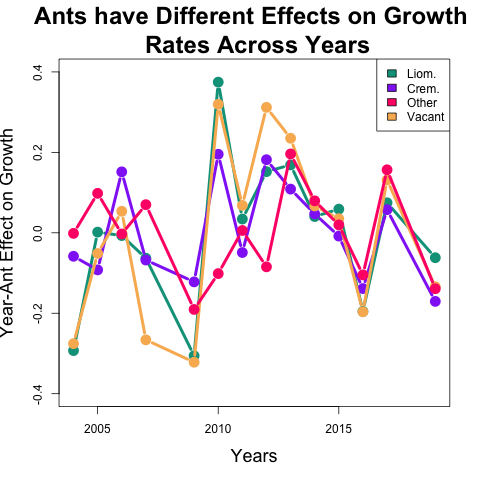
\includegraphics{"Figures/grow_year_ant_timeseries.png"}
We broke down the impacts of ant partner on the growth rate by year and found that the effects of each ant on the growth rates of the cacti don’t always align, as shown in Figure \ref{fig:year-ant}. 
In 2004, 2005, and 2007, the only ant which has a positive effect on the growth rate of the tree cholla. 
In 2006, \textit{Crem.} has the most positive effect on the growth rate of cacti, followed by Vacant, Other, and \textit{Liom.}. 
In 2007, 2008, and 2016, vacant had the most negative effect on the growth rates of cacti, while in 2012, vacant plants had experienced the most positive effects on their growth rates. 
In 2010 and 2012, the only ant which has a negative effect on the growth rate of the cacti. 
From 2013-2019, the effects of all ant partners are quite tightly coupled (all closely positive or closely negative). 

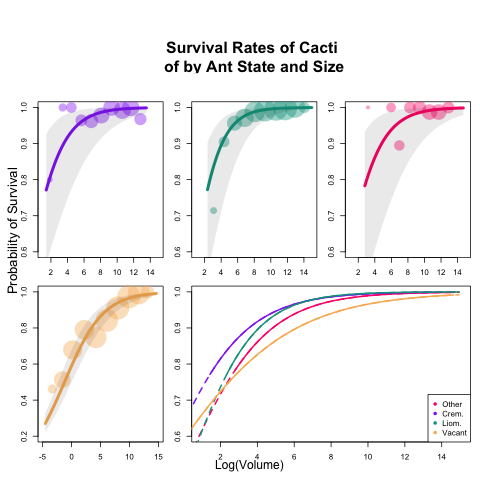
\includegraphics{"Figures/surv_panels_cropped.png"}
Our analyses of the bayesian hierarchical survival model showed that large cacti have higher survival rates than small, regardless of the ant partner. 
It also showed that small cacti had significantly different survival rates depending on the ant partner. 
Small cacti experienced highest survival rates when tended by \textit{Crem.} (near $70\%$) as compared to the lowest survival rates when tended by \textit{Liom.} or other ants (below $60\%$), as shown in Figure \ref{fig:surv}.
As tree cholla grow, the probabilities of survival increase no matter the partner to nearly $100\%$ with plants tended by \textit{Crem.} and \textit{Liom.} reaching maximum survival first and plants that are vacant reaching last. 
\textit{Crem.} tended plants have survival rates ranging from $68.379\%$ to $99.998\%$, with the rates increasing with the size of the cacti.  
\textit{Liom.} tended plants have survival rates ranging from $35.997\%$ to $99.999\%$, with the rates increasing with the size of the cacti. 
Other tended plants have survival rates ranging from $15.078\%$ to $99.999\%$, with the rates increasing with the size of the cacti. 
Vacant plants have survival rates ranging from $22.031\%$ to $99.647\%$, with the rates increasing with the size of the cacti. 

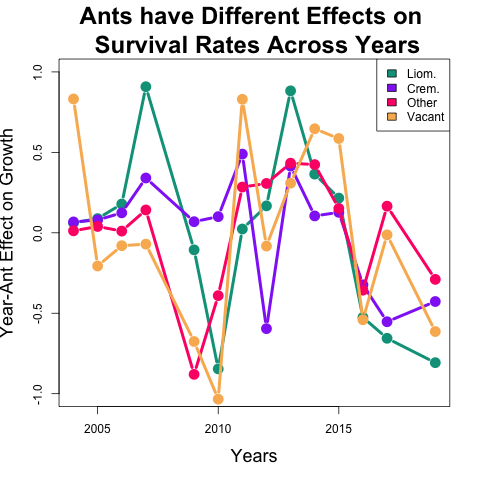
\includegraphics{"Figures/surv_year_ant_timeseries.png"}
We broke down the survival rates by year to determine the differences in ant effects across time. 
In 2004, 2011, 2014, and 2014, vacant tree cholla experienced more positive effects on their survival rates than any other cacti, while vacant cacti experienced the most negative effects on survival rates in 2005 and 2010.
In 2007 and 2013, tree cholla tended by \texit{Liom.} experienced significantly more positive effects on the survival rate than any other cacti, whereas in 2018 and 2019 \texit{Liom.} tended cacti experienced the most negative effects on the survival rates. 
In 2004 and 2009, plants tended by ants in the category of other experienced the most negative effects on survival rates, while in 2017 these plants experienced the most positive effects on the survival rates. 
\textit{Crem.} tended tree cholla experienced more negative effects on the survival rates than any other cacti. 
\textit{Crem.}, \texit{Liom.}, and Other-tended plants all experience similar patterns of positive and negative effects on survival rates through most years, with exceptions between the years of 2009-2010, 2011-2012, and 2017-2019. 

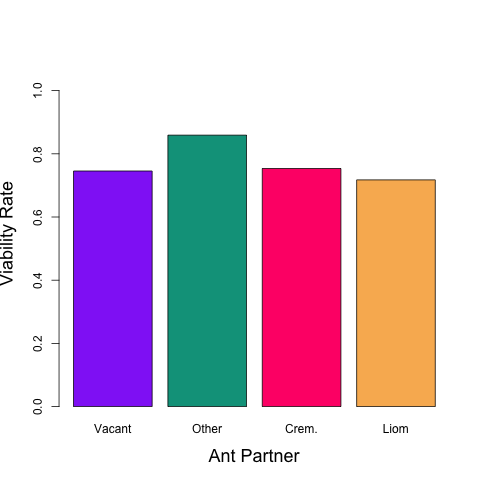
\includegraphics{"Figures/viab_bars.png"}
Tree cholla tended by \textit{Liom.} ants had significantly higher viability rates, from $79.83\%$ to $91.81\%$ with a mean of $87.047\%$, as compared to those of cacti tended by \textit{Crem.}, from $69.19\%$ to $87.60\%$ with a mean of $79,784\%$, and other, from $76.98\%$ to $86.20\%$ with a mean of $76.977\%$, as shown in Figure \ref{fig:viab}. 
The lowest observed viability rate of tree cholla flower buds ranged from $62.83\%$ to $83.78\%$ with a mean of $74.604\%$ when there were no ant partners. 
Using a chi squared test I determined that there is a $13.6\%$ chance that this difference between the mean viability rates of \textit{Liom.} tended plants and vacant plants. 

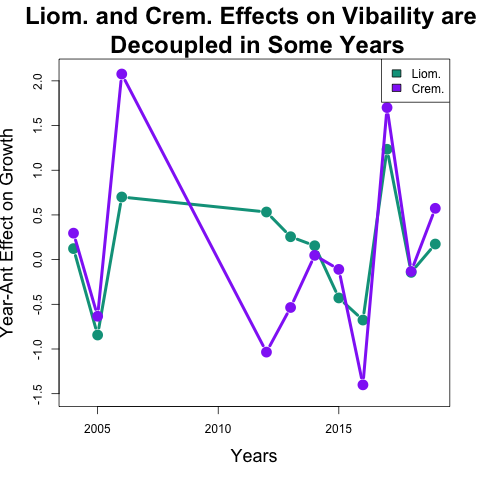
\includegraphics{"Figures/viab_year_ant_timeseries.png"}
We broke the effects of ant partners on the viability rates of cacti down by year and found that in some years the effects of different ant partners on the viability rates of the cacti are coupled while in others they differ significantly. 
IN 2004 vacant cacti experienced the most positive effects on their viability rates, whereas in 2005, vacant cacti experienced the most negative effects on their viability rates compared to other cacti. 
In 2006 and 2017, \textit{Crem.} tended cacti experienced the most positive effects on viability rates, while in 2012, 2014, 2016, and 2018, \textit{Crem.} tended cacti experienced the most negative effects on viability rates. 
In 2005,2013, 2015, and 2019, cacti tended by ants in the other category experienced the most positive effects on the viability rates, while in 2006 they experienced the most negative effects. 
In 2012, \textit{Liom} tended cacti experienced the most positive effects on their viability rates, while in 2019 they experienced the most negative. 
From the years 2013 to 2019, the effects of all ant partners on the viability rates of cacti are tightly coupled in patterns from positive to negative. 

\subsection*{Ant Transition Rates}
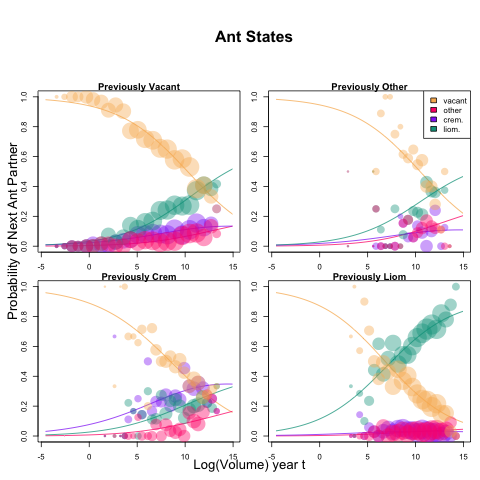
\includegraphics{"Figures/Ant_Size_Multi.png"}
All very small cacti are vacant with the probability of an ant partner increasing as the cacti grow larger, as shown in Figure \ref{fig:ant}. 
Most large tree cholla are tended by \textit{Liom.} ants even if they had a different previous partner.
The largest vacant cacti have a $42.875\%$ probability of being tended by \textit{Liom.} ants in the next season, $7.143\%$ probability of being tended by other ants in the next season, $28.571\%$ probability of being tended by \textit{Crem.}, and $21.429\%$ probability of being vacant in the next season.
Previously vacant cacti are most likely to stay vacant until the cacti reach about $10 log(m)^3$, at which point they are more likely to be tended by \textit{Liom.} ants in the next season. 
Large cacti tended by \textit{Liom.} ants are likely to be tended by \textit{Liom.} ants again ($90.476\%$) in the next season.
They have a $2.372\%$ probability of being tended by \textit{Crem.} ants in the next season, $7.143\%$ probability of being tended by other ants in the next season, and $$ probability of being vacant.  
Previously \textit{Liom.} tended cacti are most likely to be vacant until they reach the size of about $7 log(m^3)$, at which point they are most likely to be tended by \textit{Liom.} in the next season.
Only large tree cholla previously tended by \textit{Crem.} are more likely to be tended by \textit{Crem.} again than be tended by \textit{Liom.} ants in the next year. 
Large tree cholla tended by \textit{Crem.} have a $47.059\%$ probability of being tended by \textit{Crem.} in the next season, $33.333\%$ probability of being tended by \texit{Liom.} in the next season, $30\%$ probability of being tended by other ants in the next season, and $33.333\%$ probability of being vacant. 
Previously \texit{Crem.} tended plants are most likely to become vacant in the next season until they reach the size of about $15 log(m^3)$, after which they are more likely to remain tended by \texit{Crem.} ants. 
Cacti previously tended by other ants have a $24.138\%$ probability of being tended by \textit{Crem.} in the next season, $69.231\%$ probability of being tended by \texit{Liom.} in the next season, $7.692\%$ probability of being tended by other ants in the next season, and $23.076\%$ probability of being vacant. 
Medium cacti follow the same patterns as large cacti in partner transitions. 


\subsection*{Demographic Modeling}
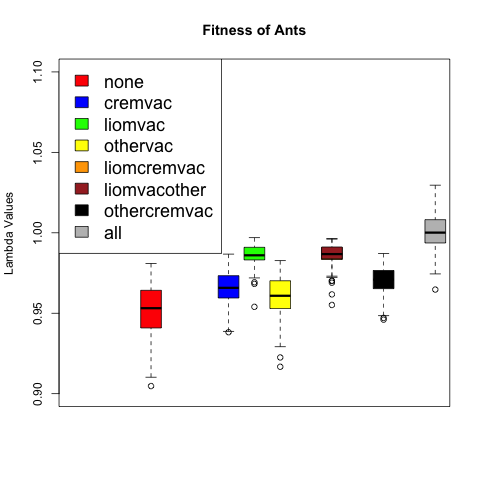
\includegraphics{"Figures/lambda_post2.png"}
We considered both a deterministic Integral Projection Model and a stochastic one to contrast the differences. 
In the deterministic model, we found that simulations with all ant partners (and vacancy) present resulted in the highest mean population growth rate while populations with no ant partners had the lowest mean population growth rate, as shown in Figure \ref{fig:lambda}.
The estimated mean population fitness of tree cholla when all ants were present was higher than the mean population fitness of any other scenario.
Similarly, only a few other scenarios had means within the interquartile range of this high partner diversity scenario. 
Honestly have no idea how much detail I should go into in this? 


\section*{Discussion}
\subsection*{Vital Rates}
\textbf{Ant partners have contrasting effects on vital rate processes of tree cholla.}
Regression analyses showed that the different ant partners had significantly different impacts on the various vital rate processes of the tree cholla cacti. 
Specifically, \textit{Crem.} tended cacti have advantages, at small sizes, over cacti tended by any other ant or vacant. 
\textit{Crem.} tended tree cholla had the highest survival rates (Figure \ref{fig:surv})  at small sizes and the highest growth rates (Figure \ref{fig:grow}), two of the most important vital rates for small cacti which are not yet reproducing. 
On the other hand, reproducing cacti which have \textit{Liom.} partners  have advantages with the highest viability rates of flower buds (Figure \ref{fig:viab}). 
Together this indicates that the best partner may change as the cacti grow and begin to reproduce, when the most vulnerable part of the plant is the flower with the seeds. 
This reflects the changes in the resource use of tree cholla as they begin to use their resources for reproduction rather than growth. 
The fact that different ant partners have significantly different effects on the various vital rates of tree cholla indicates that none of them are the “perfect” partner, and that the “best” partner may in fact change over the lifespan of the cacti. 
As the tree cholla grew, the best partner changed from \textit{Crem.} ants, partners known for ***, to \textit{Liom.} ants, partners best known for defensive benefits to the cacti, particularly against the seed predators which most impact viability. 
The difference in ant partners made a significant difference in the observed vital rates of the cacti, indicating that considering the interaction between the tree cholla and any individual partner would fail to capture the extent of the benefits to the cacti.
Like many other systems, pairwise perspectives do not fully encompass the complex impacts that multispecies mutualisms have on the focal mutualists vital rates.

\subsection*{Ant Transition Rates}
\textbf{Small cacti remain vacant, while large cacti are most likely to be tended by \textit{Liom.} ants.}
Small cacti are unlikely to be tended because most do not produce EFN, of if they do it is a very small amount. 
Medium-sized to large cacti are much more likely to be tended than vacant as they begin producing EFN, with many factors that determine the most likely partner. 
Some of the ant partners appear to have high turnover rates, meaning they are unlikely to tend the same plant multiple years in a row. 
Ants in the other category have high turnover rates, shown by the fact that medium and large cacti tended by other are unlikely to be tended by other ants again in the next season. 
The reason for these turnovers could be due to the inability to defend their territories, an ability to find and colonize new resources, or an ability to colonize resources that have been left unclaimed. 
This discovery-dominancy tradeoff is a well-studied hypothesis in ant literature \cite{lach2010} that could explain the remaining presence of ants in the other category despite high turnover rates.


On the other hand, \texit{Crem.} ants appear to have lower turnover rates, since large cacti have up to $47.059\%$ probability of being tended by \texit{Crem.} in the next year.
In addition to turnover rates, there are also colonization rates, the probability of a species taking over a cactus that was previously tended by different ants. 
\textit{Liom.} are the only ant partners we observed with high colonization rates. 
Most cacti tended by non-\textit{Liom.} ants have a high probability of being taken over by \texit{Liom} ants in the next season, as shown in Figure \ref{fig:ant}.
This pattern could be due to the well-known high levels of aggression displayed by \textit{Liom.} ants in this system, however there are other possible explanations, such as nectar composition.
The exception to this rule are plants tended by \textit{Crem.} ants which are more likely to remain tended by \textit{Crem.} than be taken over by \textit{Liom.} in the next season. 
The trend that most large ants are likely to be tended by \textit{Liom.} ants reflects the findings that large cacti benefit most from \textit{Liom.} as ant partners. 
As explained in the introduction, there are many factors that determine the colonization rates of different cacti by their ant partners, including EFN quantity and quality, ability to seek out cacti, aggression, and more.
These patterns could be explained by the \textit{Liom.} ants ability to dominate at a resource site and therefore takeover from different ants which originally found the site. 


An alternative, or parallel, explanation for these ant transitions could be the changes in EFN composition across ontogeny of the cacti.
As cacti grow the chemistry of EFN produced changes\cite{Miller2013}, changing from more *** composition to *** composition. 
Different ants have preferences for different nectar compositions\cite{Lach2010}, specifically, ***.
This could provide a potential route for the cacti to select their own ideal partners
This indicates a potential future avenue of research into the correlations between ant partners and the chemistry of the EFN produced by the tree cholla. 

\subsection*{Demographic Modeling}

	
\end{document}

\typeout{\bibliography{References.bib}}
